\documentclass[11pt]{beamer}
\usepackage{hyperref}
\usepackage[czech]{babel}
\usepackage[utf8]{inputenc}
\usepackage{graphics}
\usepackage{listings}
\usetheme{Darmstadt}
\usecolortheme{wolverine}
\setbeamertemplate{footline}[frame number]      

\title{Řadící algoritmy - Řazení záměnou}
\author[Václav Doleček]{Václav Doleček\\
{\small \href{xdolec03@stud.fit.vutbr.cz}{\texttt{xdolec03@stud.fit.vutbr.cz}}}}
\institute[VUT]{Vysoké učení technické \\ Fakulta informačných technológií}
\date{\today}

\begin{document}
 
\frame{\titlepage}

 
\begin{frame}[fragile]{Řadící algoritmy}
\begin{center}
    "Řadící nebo třídící algoritmus zajišťuje uspořádání dané monižiny prvků(pole, seznamu, souboru) do požadovaného pořadí."\footnote{\tiny\href{https://en.wikipedia.org/wiki/Sorting_algorithm}{Zdroj: Wikipedie}}
\end{center}

Řadící algoritmy jsou klasifikovány dle:
\begin{itemize}
    \item[\(\Rightarrow\)] Použití paměti
    \item[\(\Rightarrow\)] Složitosti
    \item[\(\Rightarrow\)] stability a adaptivnosti
    \item[\(\Rightarrow\)] Sériové nebo paralerní
\end{itemize}
Výstup jakéhokoliv Řadícího algoritmu musí být:
\begin{itemize}
    \item[\(\Rightarrow\)] Permutací vstupní množiny
    \item[\(\Rightarrow\)] Seřazeny dle klíče, či pořadí
\end{itemize}

\end{frame}




\begin{frame}[fragile]{Bubble sort algoritmus - Definice}
\begin{itemize}
    \item Bubble sort je jeden z~nejjednodušších řadících algoritmů, který pracuje na principu stáleho přehazování sousedících prvků, pokud jsou ve \underline{špatném pořadí}.
    \\
    \
    \item Množinou prochází opakovaně dokud není uplně seřazena (dokud nedojde při průchodu ani jednomu prohození)
    \\
    \
    \item S~porovnání s~ostatními je tento algoritmus pomalý, používá se hlavni pro téměř seřazené množiny\footnote{\tiny\href{https://en.wikipedia.org/wiki/Bubble_sort}{Zdroj: Wikipedie}}
\end{itemize}

    
\end{frame}
 
\begin{frame}{Demonstrace}
\begin{center}
( \underline{4} \underline{1} 2 5 8 ) \(\rightarrow\) ( \underline{1} \underline{4} 2 5 8 ) ; 4 $>$ 1 prohodil\\

( 1 \underline{4} \underline{2} 5 8 ) \(\rightarrow\) ( 1 \underline{2} \underline{4} 5 8 ) ; 4 $>$ 2 prohodil\\

( 1 4 \underline{2} \underline{5} 8 ) \(\rightarrow\) ( 1 4 \underline{2} \underline{5} 8 ) ; správné pořadí\\

( 1 4 2 \underline{5} \underline{8} )  \(\rightarrow\) ( 1 4 2 \underline{5} \underline{8} ) ; správné pořadí\\
\end{center}

\begin{itemize}
    \item[\(\Rightarrow\)]<1-> Pokud je větší číslo před menším, prohodí se jejich místo
    \item[\(\Rightarrow\)]<2-> Pokud je menší číslo před větším, nebo jsou stejné, jejich místa se neprohazují
    \item[\(\Rightarrow\)]<3-> Pruchod přes množinou se opakuje do té doby, dokud nedojde k~jediné záměně prvků\footnote{\tiny\href{https://en.wikipedia.org/wiki/Bubble_sort}{Zdroj: Wikipedie}}
\end{itemize}
\end{frame}


\begin{frame}[fragile]{Grafická demostrace}

\begin{figure}[]
        \centering
        \scalebox{0.3}{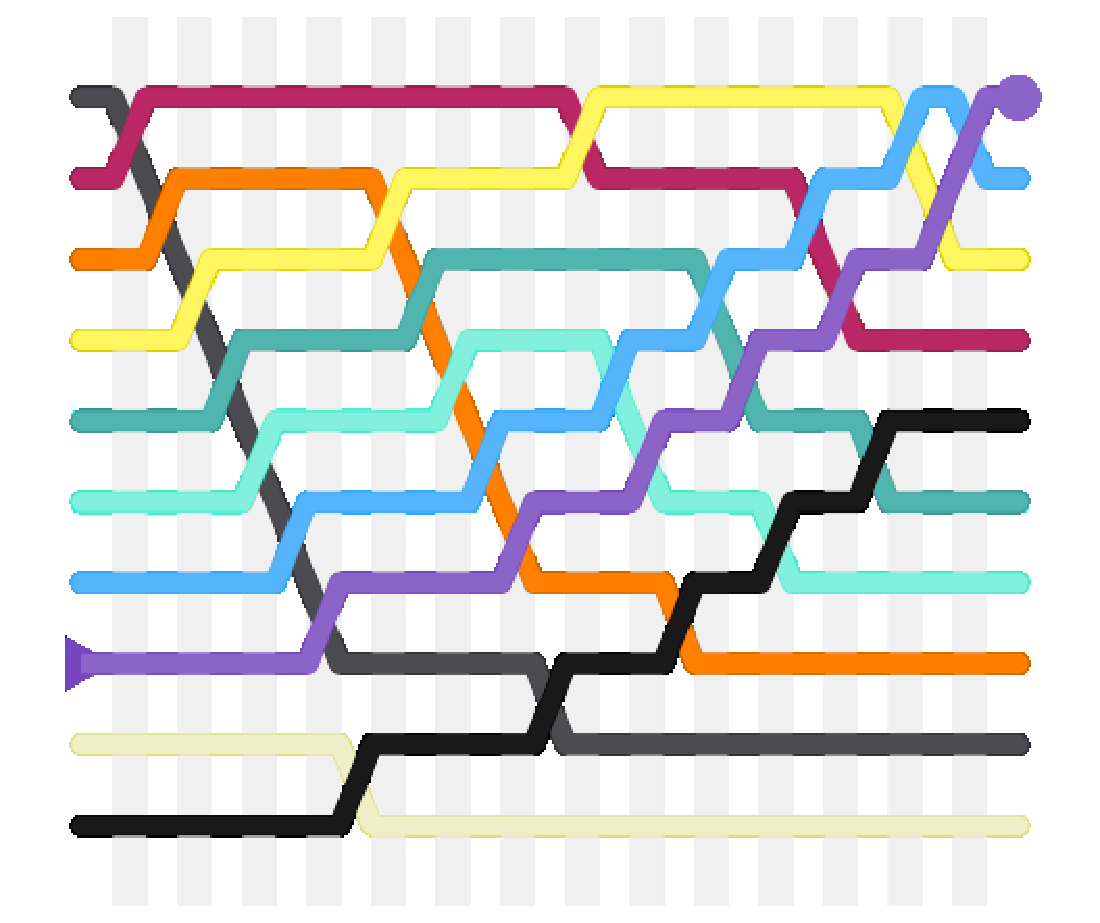
\includegraphics{Bubble_sort.eps}}
    \end{figure}
\begin{itemize}
    \item Barevný diagram bublinkového řazení - barva označuje prvek řazené posloupnosti, zleva doprava sledujeme možný průběh řazení\footnote{\tiny\href{https://en.wikipedia.org/wiki/Bubble_sort}{Zdroj: Wikipedie}}
\end{itemize}
\end{frame}

\begin{frame}[fragile]{Pseudo kód}
\begin{itemize}
    \item Toto je jedna z~mnoha variací algoritmu:\footnote{\tiny\href{https://tiny.cc/dt6i7y}{Zdroj: Wikipedie}}
\end{itemize}
\begin{verbatim}
 limit := počet_prvků;
   opakuj
       bylo_seřazeno := ano;
       limit := limit - 1;
       pro i od 1 do limit opakuj:
           pokud seznam[i] > seznam[i + 1]
               zaměň(seznam[i], seznam[i + 1])
               bylo_seřazeno := ne;
   dokud není bylo_seřazeno == ano nebo limit == 1;
\end{verbatim}

\end{frame}

\begin{frame}{Konec a zdroje}

Wikipedie:

\(\Rightarrow\)\;\url{https://en.wikipedia.org/wiki/Sorting_algorithm}
\(\Rightarrow\)\;\url{https://en.wikipedia.org/wiki/Bubble_sort}
\(\Rightarrow\)\;\url{https://tiny.cc/dt6i7y}

\medskip
Geeks for Geeks:

\(\Rightarrow\)\;\url{https://www.geeksforgeeks.org/bubble-sort/}



\end{frame}
\end{document}
